%!TEX root = paper.tex
%%%%%%%%%%%%%%%%%%%%%%%%%%%%%%%%%%%%%%%%%%%%%%%%%%%%%%%%%%%%%%%%%%%%%%%%%%%%%%%%
\section{Conducting Measurements}
\label{sec:measurementgoals}


% ripped from previous game mechanics section
% basis for new simulation section
\begin{figure}[!t]
	\centering
	%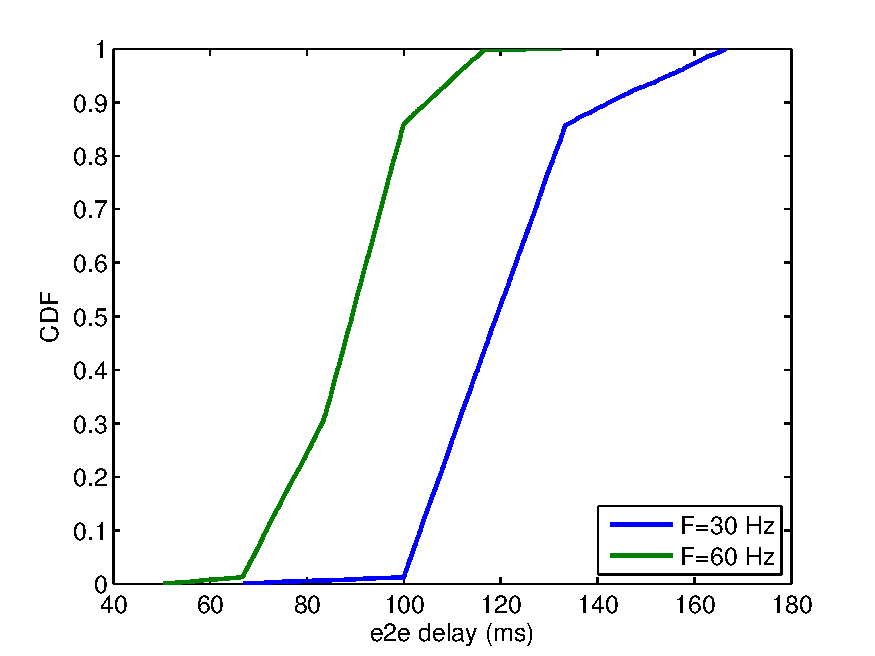
\includegraphics[width=1.0\columnwidth]{images/e2e-delay-sim.pdf}
	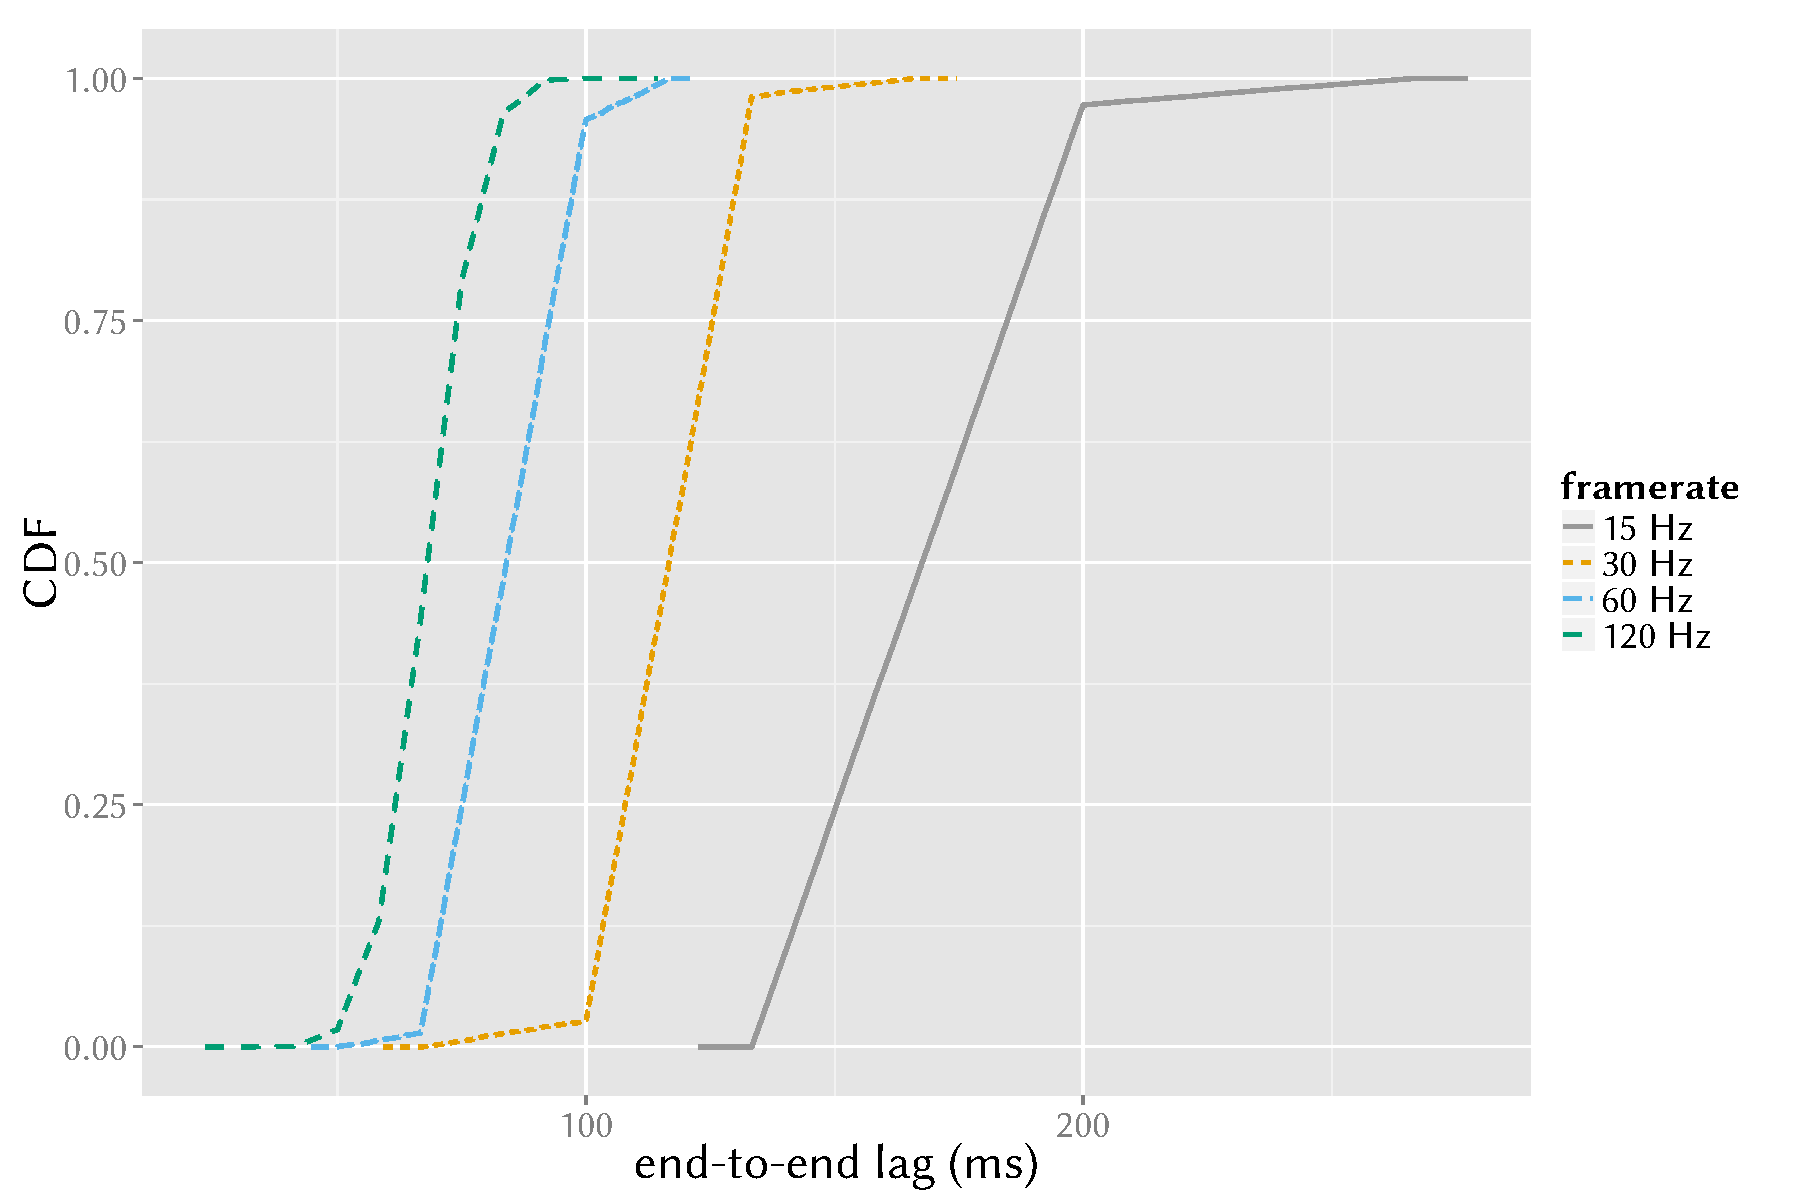
\includegraphics[width=1.0\columnwidth]{../simulation/visualization/matlab-framerate-lag.pdf}
	\caption{\acrshort{ECDF} of a simulated online video game interaction and the resulting end-to-end lag depending on the game's frame rate. One-way network delay followed a Gaussian distribution with $\mu = \SI{20}{\milli\second}$ and $\sigma = \SI{5}{\milli\second}$. The server's tickrate was set to \SI{60}{\hertz}.}
\label{fig:e2e-delay-sim}
\end{figure}



\begin{figure}[!t]
	\centering
	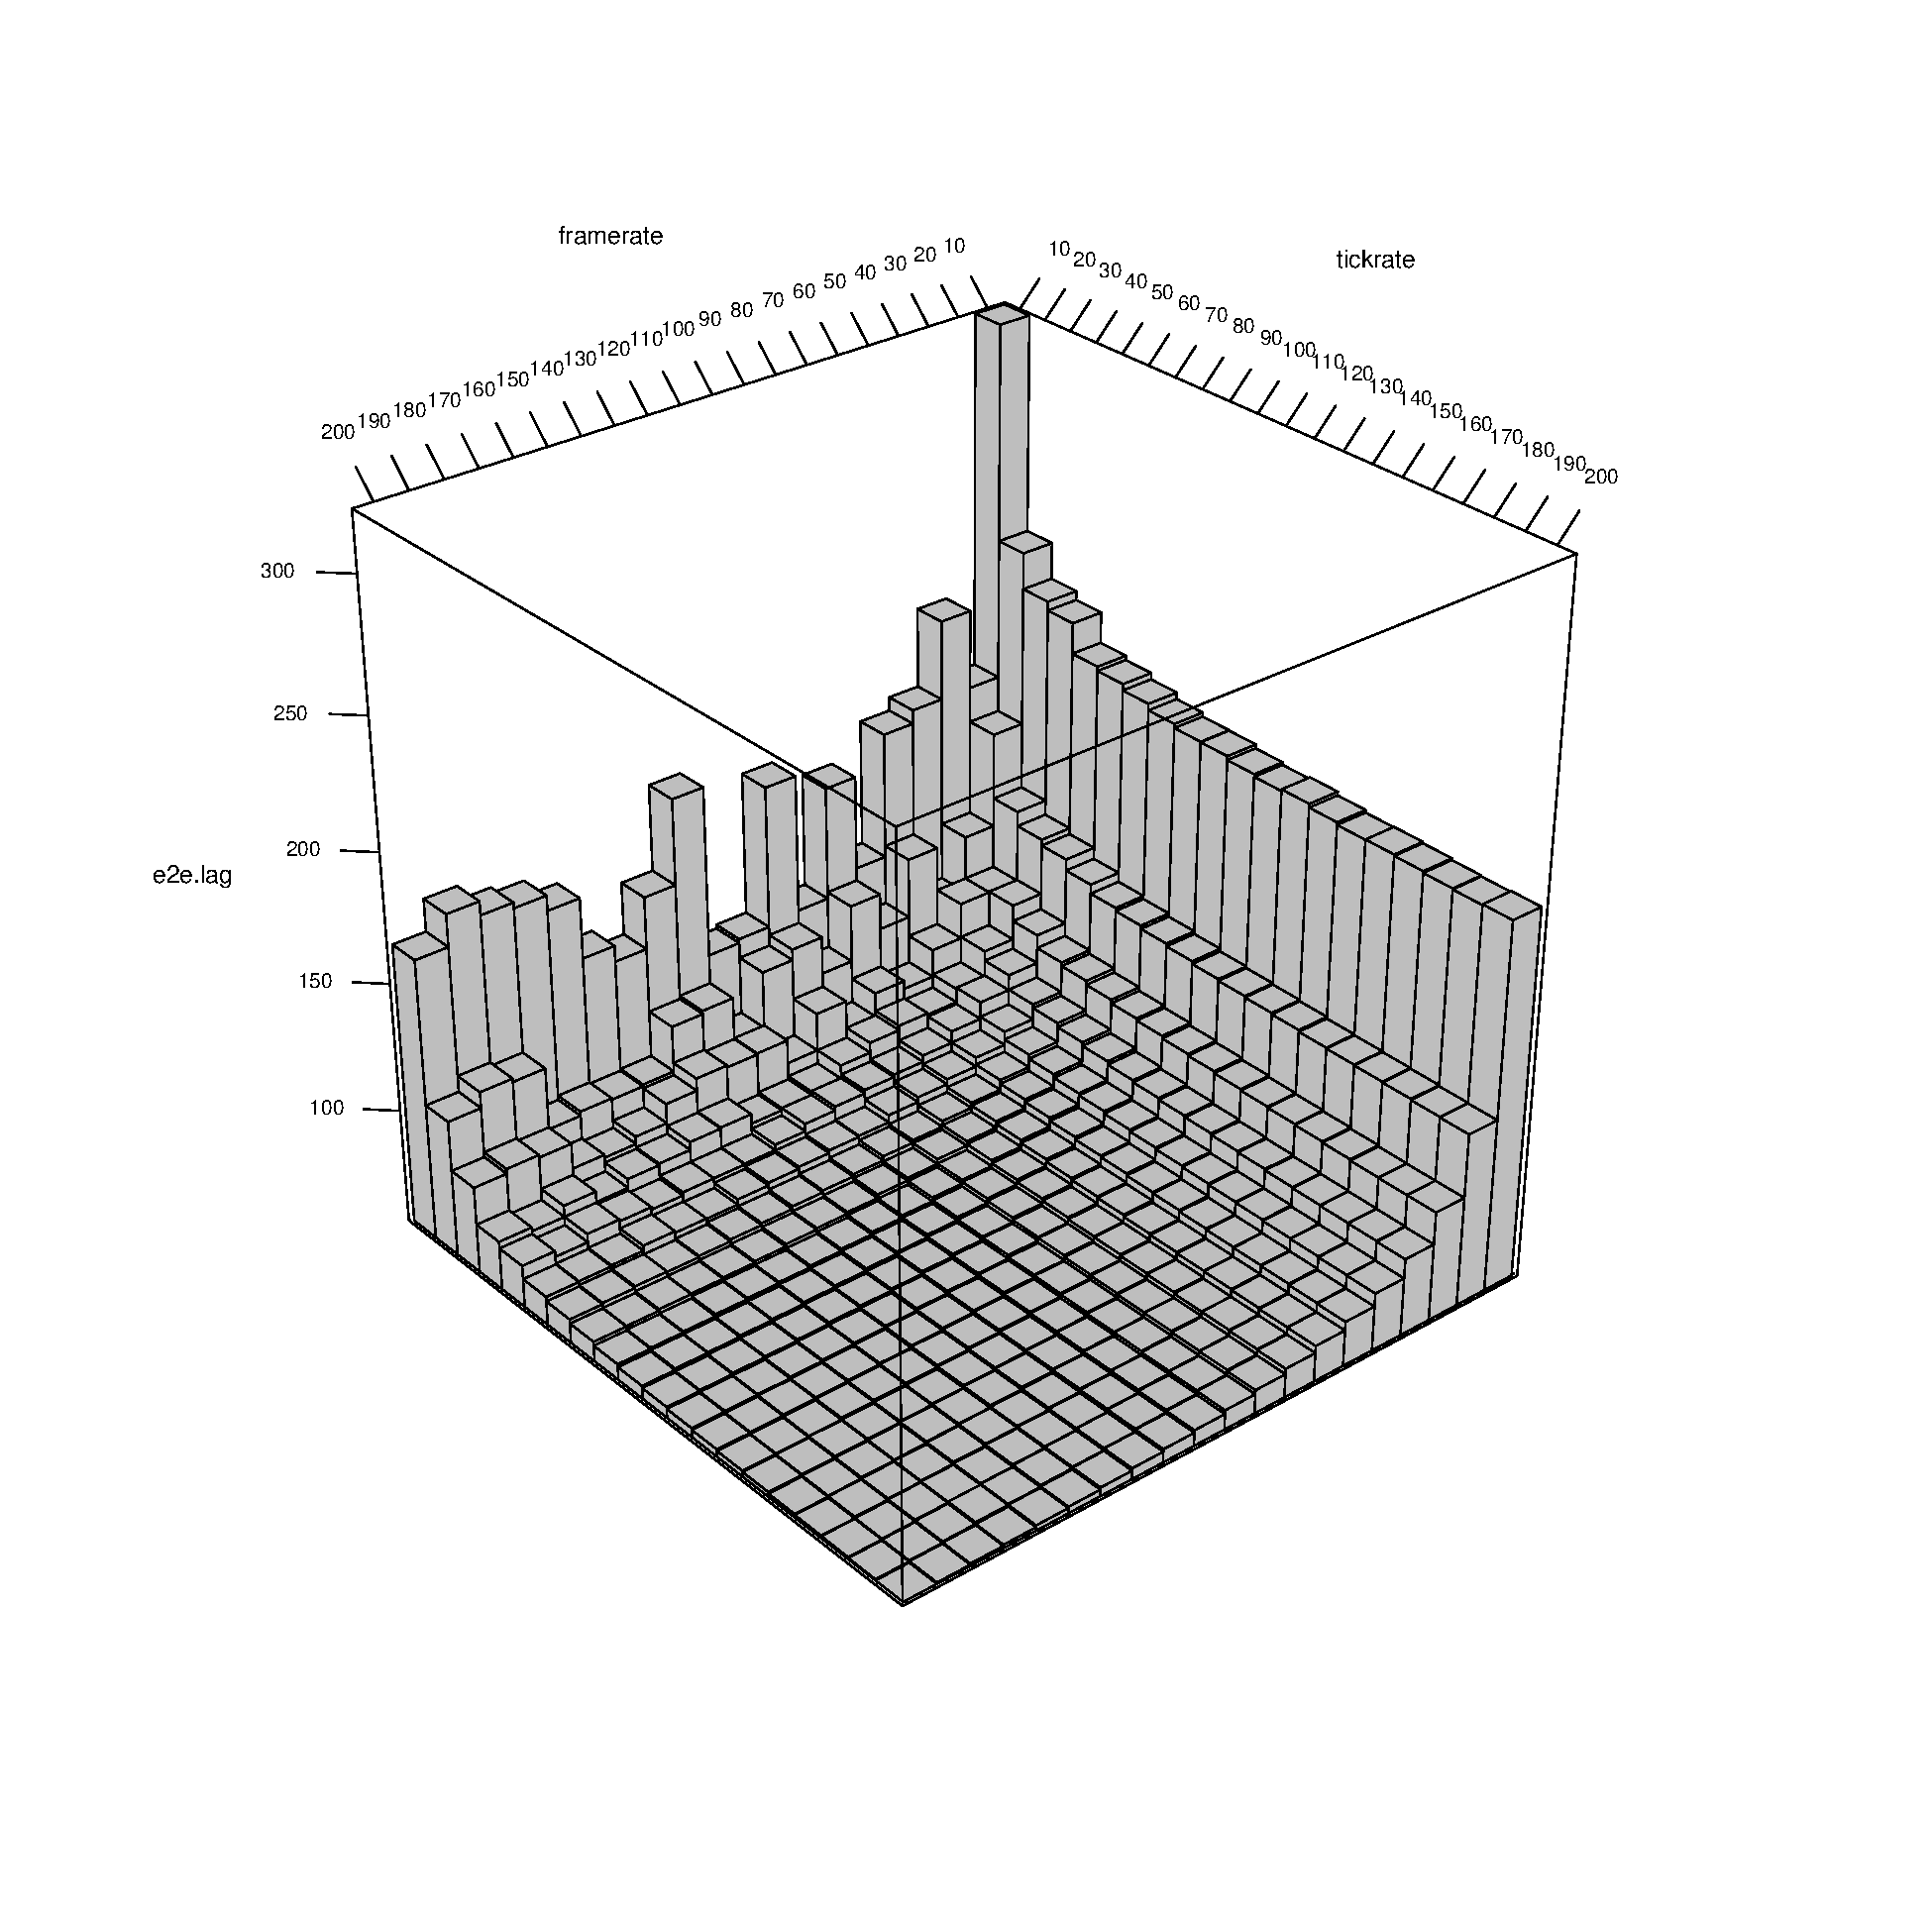
\includegraphics[width=1.0\columnwidth]{../simulation/visualization/e2e-lag-3dbars.pdf}
	\caption{Process model of TODO.}
\label{fig:3dbars-framerate-tickrate-lag}
\end{figure}

Before proposing actual measurement methods, three equally important aspects relating to any game measurement approch are discussed: the metrics to evaluate, the parameters to use, as well as the selection of games. 

Finding fitting objective \gls{QoE} metrics is strongly game-dependent. They need to reflect the game's mechanics in a meaningful manner. But this is beyond the scope of this paper, which will only concern itself with game-independent metrics, of which three are considered here: The framerate, the frame \gls{IAT}, and the end-to-end lag (or parts thereof as some measurement methods might not be able to record the full lag).

The framerate and \gls{IAT} are a good representation for the game's fluidity and responsiveness to inputs and are especially important to note for cloud gaming. The end-to-end lag gives the best overall picture on the attainable gaming experience and should always be preferred over partial lag values, such as purely investigating the network latency. The impact of the lag also depends on the type and precision of controls the game offers. A keyboard and mouse driven PC game might be much more sensitive to high lag than a mobile game with touch controls.

Input controls are but one aspect of the games environment and settings, which also need to be carefully selected to achieve meaningful results. This especially concerns PC games which usually offer a wide range of options to choose from of which the graphics options are the most impactful. The recommended settings to run games at are a video resolution of 1080p or higher with the games other graphics options set to high or at lest medium values in order to reflect a typical gaming experience. The test computers should be able to deliver these graphical settings at a framerate of \SI{60}{\hertz} which is considered the minimum rate for many players. Some types of games are less dependent on the framerate, where a rate of \SI{30}{\hertz} is considered acceptable. Experimenters should never set a framerate lower than that for the reasons discussed in the previous section. They should however also consider testing at higher framerates, especially for competitive games with a high tickrate to further reduce the negative impact of low framerates.


%%%%%%%%%%%%%%%%%%%%%%%%%%%%%%%%%%%%%%%%%%%%%%%%%%%%%%%%%%%%%%%%%%%%%%%%%%%%%%%%
\subsection{Choosing Representative Games}
\label{sec:game-criteria}

%The general focus here lies on measuring online games with high demands. The idea is that if these games work at an objectively good quality, it is reasonable to assume that all other games do so as well. 
It is quite difficult to find games that are representative for certain input and lag demands. For example, the traditional game genre categorization is not a good starting point as games from the same category can be vastly different in terms of game speed and necessary reaction times. Rather, the following four metrics might be more helpful to assess a game's applicability for measurements.

 \begin{itemize}
    \item \textbf{Required number of decisions or actions in a certain time span.} E.g., the \gls{CCG} \textsc{Hearthstone} may only require a handful of actions (i.e., choosing and playing cards) each turn, while in order to competitively play the \gls{RTS} \textsc{Starcraft 2} you more or less need to achieve a few hundred so-called \gls{APM}, with the record being higher than $800$ \gls{APM}.% \cite{6404025} defines a related metric dubbed \textit{command heaviness} comparing the amount of change to the input rate, under the umbrella term \textit{real-time strictness}. This ties in with the concepts of game sense. Micromanagement-intense games usually tend to result in high APM rates.

    \item \textbf{Maximum successful reaction time to in-game actions.} Again e.g., \textsc{Hearthstone} as a turn-based game requires no instant reaction time at all, as the opponent's and the player's actions are separated into turns. First-person shooters like \textsc{Counter-Strike: Global Offensive} are usually on the opposite extreme of this spectrum, as they tend to have a very high tickrate and literally often require you to ``shoot first'' to win. This is also investigated/defined in \cite{Claypool:2006:LPA:1167838.1167860}. This metric is also closely related to the next item.

    \item \textbf{(Un-)Predictability of actions.} Compare, e.g., an entirely rhythm-based game (e.g., \textsc{Guitar Hero}), where you can completely pre-plan all of your actions, to a twitch-based shooter like \textsc{Counter-Strike} where you have to react from moment to moment. In theory, a game with no surprising events will be much less influenced by a higher end-to-end lag.

    \item \textbf{Accuracy and precision of input actions.} Accuracy can be both in terms of temporal as well as spatial aspects which can be influenced by both the image quality and the frame rate.  %Commands through keybindings usually require less precision than freeform mouse inputs on certain regions on the screen.

\end{itemize}


%%%%%%%%%%%%%%%%%%%%%%%%%%%%%%%%%%%%%%%%%%%%%%%%%%%%%%%%%%%%%%%%%%%%%%%%%%%%%%%%
%%%%%%%%%%%%%%%%%%%%%%%%%%%%%%%%%%%%%%%%%%%%%%%%%%%%%%%%%%%%%%%%%%%%%%%%%%%%%%%%
\subsection{Measurement Approaches}
\label{sec:measurementapproaches}

With these metrics, test parameters, and categorizations in mind, one can now attempt to conduct the actual measurements of which there are three distinct methods each situated at a unique vantage point as depicted in Fig.~\ref{fig:measurement-methods}.

\begin{figure}[!t]
    \centering
    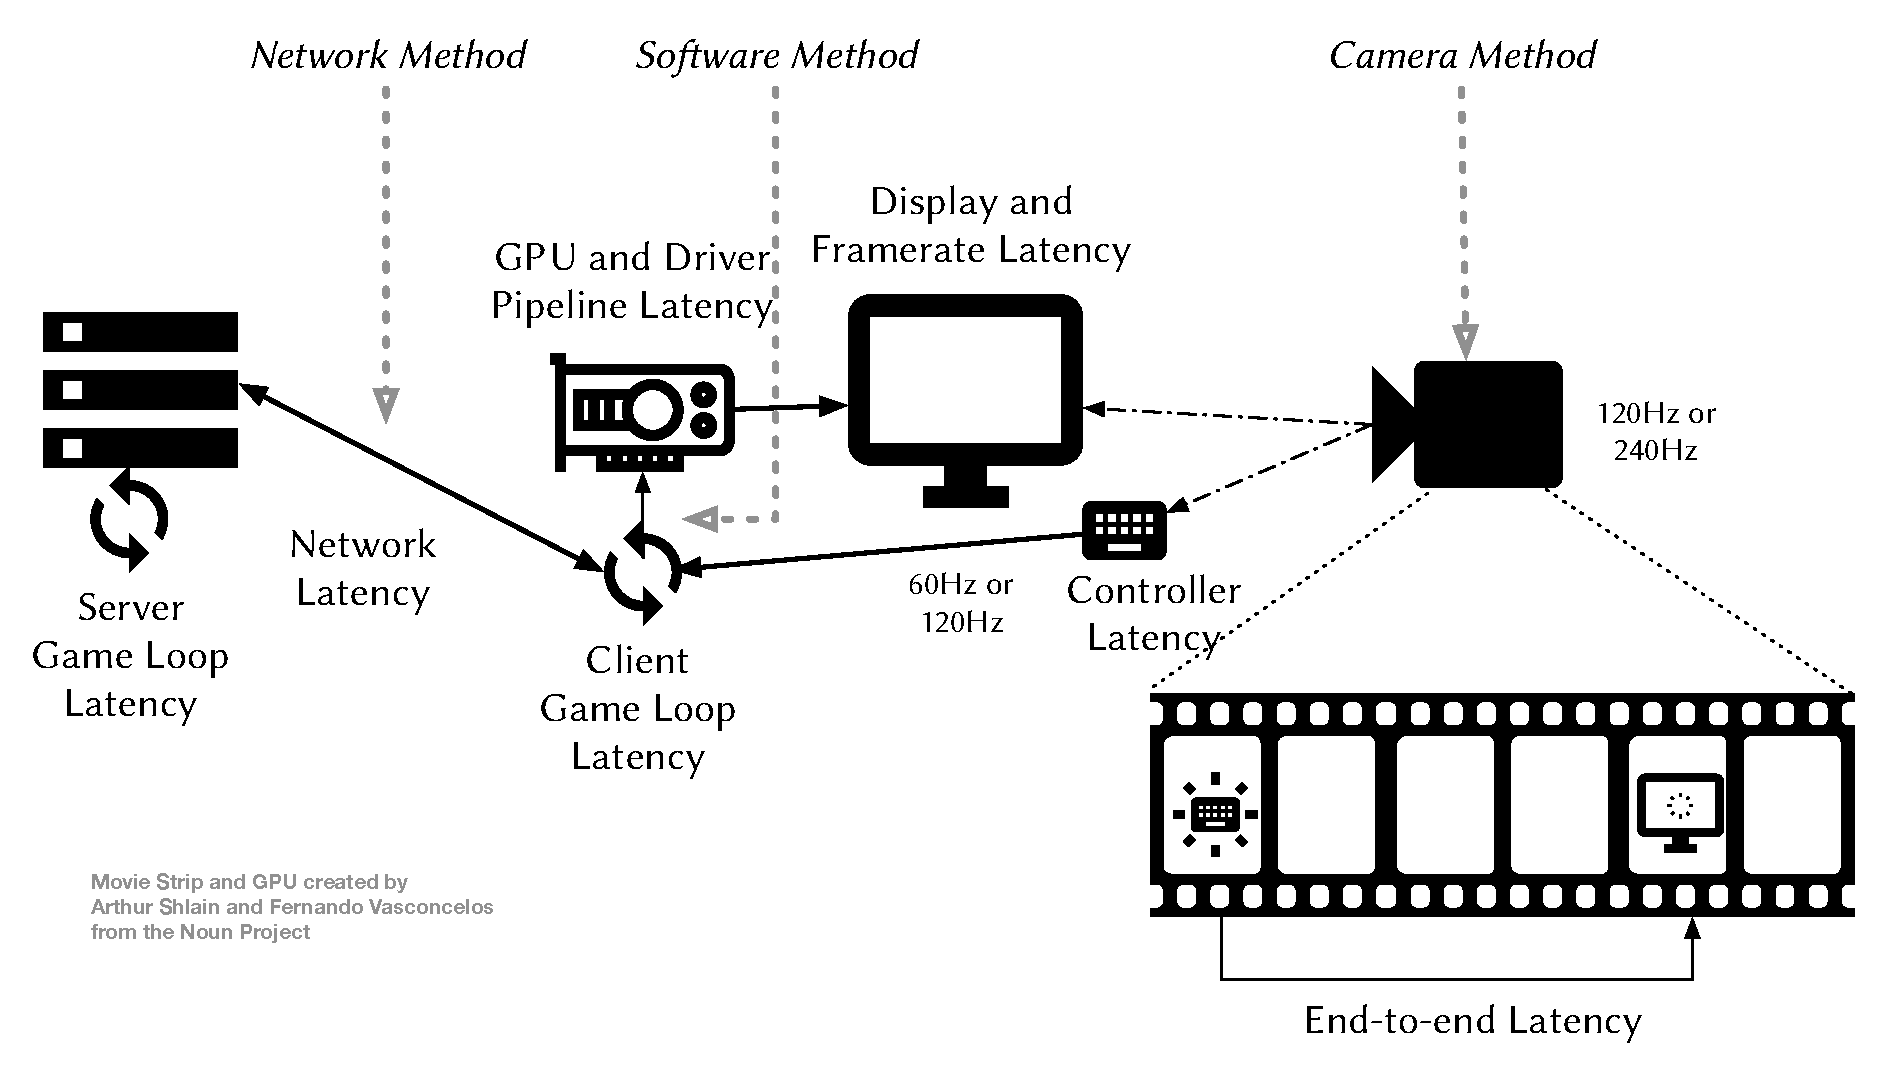
\includegraphics[width=1.0\columnwidth]{../models/e2e-lag.pdf}
    \caption{Location of the three measurement approaches to capture end-to-end latency inside a usual online video game lag chain.}
\label{fig:measurement-methods}
\end{figure}


%%%%%%%%%%%%%%%%%%%%%%%%%%%%%%%%%%%%%%%%%%%%%%%%%%%%%%%%%%%%%%%%%%%%%%%%%%%%%%%%
\subsubsection{Screen Recording Software Method}

Recording the output stream of a video game might be the simplest approach. It can capture both the framerate and \gls{IAT} at a driver level, and the recorded video can be used for image and quality analyses as well as to correlate it to additionally recorded input events to calculate the lag. This is not the the complete end-to-end lag however, as both the controller and screen output latency are missing. The need to install additional software might make it unsuitable for some scenarios, e.g., when measuring console video games. As a variant of this method, one can also record the output stream with a video capture card on a secondary computer, which does not negatively effect the game's performance as the software method does.

Examples of this approach include both \cite{Chen:2011:MLC:2072298.2071991} and \cite{6670099} which measured the end-to-end latency of cloud gaming services in the game client. They do this by invoking the system menu in games and measuring the time until it is displayed. A 2013 paper \cite{6574660} investigates the quality of cloud gaming interactiveness (i.e., the lag) as well as image quality by employing software recording methods on the client's computer.
%However, this method assumes a constant delay of game actions and may not capture the actual end-to-end lag of many of real game actions, as they are typically different from and longer as the latency of displaying a menu. A 2013 paper \cite{6574660} investigates the quality of cloud gaming interactiveness (latency) as well as image quality by employing software recording methods on the client's computer. With these techniques the challenges regarding the quality are discussed.


%%%%%%%%%%%%%%%%%%%%%%%%%%%%%%%%%%%%%%%%%%%%%%%%%%%%%%%%%%%%%%%%%%%%%%%%%%%%%%%%
\subsubsection{Passive Network Measurements}

In some cases it may also be advantageous to tap into the network interactions of the games and record the command and update messages sent between server and clients. While this is not a direct measure of game quality, it can give insights into the game's inner workings, such as the tick rates, and one can derive, e.g., the lowest achievable end-to-end lag from this.

%Can only investigate command and update messages, not tick rate directly. Evaluate rate, IAT, and bandwidth, estimate latency (though there may be no direct link between commands and updates).

Besides simple flow-based or packet-counting network metrics, many games also allow for deeper packet-dissecting analyses, as the often rely on standardized protocols or data formats, such as Protobuf\footnote{\url{https://developers.google.com/protocol-buffers/}} or incorporate well-known third-party multiplayer-enabling libraries. %And cloud games sometimes use derivates from the RTP-family or XMPP-based(VERIFY) protocols. 
Additionally, almost no game encrypts its time-critical messages, enabling an easy read-out. Through these means, the specific commands can be read from the network and potentially linked to their effect on the game state in the corresponding state update messages.
%, but also potentially allowing malicious actions to be taken easily.


%%%%%%%%%%%%%%%%%%%%%%%%%%%%%%%%%%%%%%%%%%%%%%%%%%%%%%%%%%%%%%%%%%%%%%%%%%%%%%%%
\subsubsection{Camera Recordings}

The only method to fully capture the end-to-end lag is to simultaneously record both the screen and input device through an external camera. The experimenter then has to count the frames between pressing a button on the input device and the action appearing on the screen and calculate the lag from this. For better visibility the input device is usually modified with an LED that turns on when the button is pressed. Also, the camera should operate at least at twice the monitor's refresh rate according to the Nyquist-Shannon sampling theorem. An additional benefit of this method is, that the game and the computers remain unaltered and are therefore not affecting any game mechanics. This approach is often used in the gaming press and by game developers to evaluate a game's control fidelity. A variant of this approach, replacing the camera with a photodiode and synthetically creating the input events with a microcontroller is described in \cite{beyermethod}, though it may be difficult to use for certain game actions that have a barely visible or unpredictable on-screen effect.


% Ultimately, to capture any and all latency sources in gaming you would need to rely on external recording gear.
% With modified input: zero latency and visible input detection (e.g. solder some LEDs to the buttons)

% Also Arduino with photodiode method described in \cite{beyermethod}
% Both this and camera method also work for closed game consoles


%%%%%%%%%%%%%%%%%%%%%%%%%%%%%%%%%%%%%%%%%%%%%%%%%%%%%%%%%%%%%%%%%%%%%%%%%%%%%%%%
%\subsection{Evaluated Metrics}

%%%%
%\subsubsection{Frame Rates and Frame Times (i.e. frame IAT)}
%i.e. frame IAT
%Reasoning for frame IAT and the negligence of past investigations
%%%%
%\subsubsection{Total and additional end-to-end latency}
%physical controller input to in-game reaction
%different in-game actions have already difference in latency, therefore need to test various actions for a complete picture
%Also discuss RTT as Hz (1/RTT) as measure for interactivity


%%%%%%%%%%%%%%%%%%%%%%%%%%%%%%%%%%%%%%%%%%%%%%%%%%%%%%%%%%%%%%%%%%%%%%%%%%%%%%%%
%\subsection{Reasonable Configuration/Setting Ranges to Test}

% Resolution: Minimum 720p, 1080p recommended, even higher is better (1440p or 2160p)
% Frame rate: 60 fps very much recommended, 30 absolute minimum,  120 or 144 can also be feasible
% Configure games to run at high or at least medium settings
% For console games: use the games intended settings for the console, never downscale the game or reduce the frame rate for streaming
% Assume no network latency higher than 200ms, preferably less than 100ms
% Assume typical access link conditions, i.e. no less than 10-16Mb/s



%Works only for general purpose computing devices with full access.
%Easiest method, but might not capture full end-to-end latency.
%FRAPS, OBS, DirectX Hooking, MSI Afterburner
%FCAT as hybrid solution with external capture card and computer


% \url{http://www.red.com/learn/red-101/high-frame-rate-video}


% articles:
% why frametimes
%     \url{https://techreport.com/review/21516/inside-the-second-a-new-look-at-game-benchmarking}

% Inside the second with Nvidia's frame capture tools
%     \url{https://techreport.com/review/24553/inside-the-second-with-nvidia-frame-capture-tools}

 % As the second turns: the web digests our game testing methods
 %    \url{https://techreport.com/blog/24133/as-the-second-turns-the-web-digests-our-game-testing-methods}

% GPU Reviews: Why Frame Time Analysis is important
%     \url{http://www.vortez.net/articles_pages/frame_time_analysis.html}

% Durante's Witcher 3 analysis: the alchemy of smoothness
%     \url{http://www.pcgamer.com//durantes-witcher-3-analysis-the-alchemy-of-smoothness/}


% Analysing Stutter – Mining More from Percentiles
%     \url{https://developer.nvidia.com/content/analysing-stutter-%E2%80%93-mining-more-percentiles-0}

% fraps vs fcat method
%     \url{http://www.extremetech.com/gaming/154089-after-almost-20-years-gpu-benchmarking-is-moving-past-frames-per-second}

% FRAPS + FRAFS
% \url{http://www.fraps.com/}
% \url{http://sourceforge.net/projects/frafsbenchview/}
% \url{http://www.5group.com/wordpress/2012/07/14/gpu-mist-pre-release-1-0-rc1/}

% issue: Fraps measures the flip queue input rather then the actual render output frames which is fine when measuring FPS but is rather poor if you want to measures actual frame times and analyze microstutter.


% NVIDIA FCAT
% \url{http://www.geforce.com/hardware/technology/fcat}
% \url{http://www.overclockers.com/nvidias-fcat-gpu-testing-pursuing/}


% Valve for Linux GL Games
% \url{https://github.com/ValveSoftware/voglperf}

% Info über MSI Afterburner overlay? oder GF experience? GPU-Z? Rivatuner Statistics Server?
% \url{http://www.overclock.net/a/how-to-use-rivatuner-afterburner-on-screen-display-and-more}



% \url{https://en.wikipedia.org/wiki/Game_classification}
% \url{https://en.wikipedia.org/wiki/Video_game_genre}
% \url{https://en.wikipedia.org/wiki/List_of_video_game_genres}

